\section{Proprietà generalizzate dei sistemi}

I modelli relativi a sistemi anche molto diversi fra loro hanno proprietà che possono essere caratterizzate dalla stessa espressione matematica. Ognuno di noi è familiare col concetto della resistenza elettrica ($R$) definita dalla legge di Ohm come: 
$$V = RI$$ 
dove $V$ è il voltaggio, o differenza di potenziale, ai capi del resistore e $I$ rappresenta la corrente che fluisce attraverso di esso. Notate che $V$ è una variabile ``ai capi'' e rappresenta una misura della \textit{forza} elettrica applicata; $I$ è una variabile ``attraverso'' e rappresenta una misura di \textit{flusso} di carica. Se ora definiamo con $\psi$ una variabile di forza generalizzata e con $\zeta$ una variabile di flusso generalizzato, la legge di Ohm diventa:
$$\psi = R \zeta $$
in cui $R$ rappresenta ora una resistenza generalizzata. La \figurename~\ref{generalized} mostra questo concetto di resistenza generalizzata applicato a diversi tipi di sistemi. Nello smorzatore meccanico, quando ai suoi capi è applicata una forza $F$, si ha un allungamento con una velocità $v$ proporzionale a $F$. Se facciamo corrispondere $F$ e $v$ rispettivamente a $\psi$ e $\zeta$ otteniamo nuovamente la legge di Ohm generalizzata. La costante di proporzionalità $R_m$, che è correlata alla viscosità del fluido all'interno dello smorzatore, fornisce una misura della resistenza meccanica alla quale ci si riferisce col termine \textit{coefficiente di smorzamento}. In fluidodinamica la legge di Ohm generalizzata assume la forma della legge di Poiseuille, la quale afferma che il flusso volumetrico di fluido $Q$ attraverso un condotto rigido è proporzionale alla differenza di pressione $\Delta P$ ai capi del tubo; la resistenza fluidodinamica $R_f$ è direttamente proporzionale alla viscosità del fluido e alla lunghezza del condotto e inversamente proporzionale alla potenza quarta del raggio. Nella legge di trasmissione del calore di Fourier il flusso di calore $Q$ condotto attraverso un dato materiale è direttamente proporzionale alla differenza di temperatura $\Delta T$ ai capi della stessa. Si può mostrare che la resistenza termica $R_t$ è in relazione con l'inverso della \textit{conduttanza termica} del materiale. Infine, nei sistemi chimici il flusso $\phi$ di un soluto attraverso una membrana permeabile è proporzionale alla differenza di concentrazione $\Delta C$ del soluto fra i capi della membrana. La resistenza al flusso chimico $R_c$ è inversamente proporzionale alla \textit{diffusività}.
\begin{figure}[htb]
	\centering
	\subfigure[]%
	{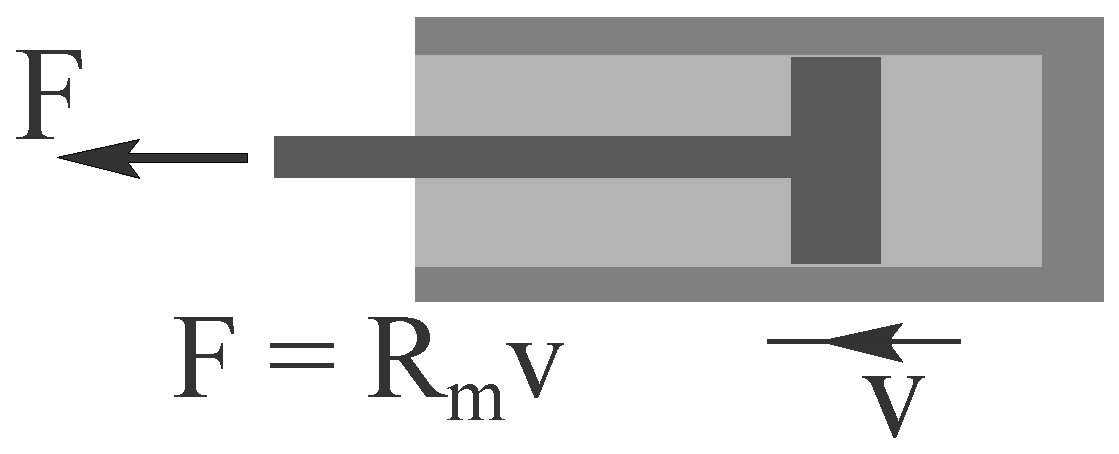
\includegraphics[width=0.35\textwidth]{immagini/dashpot.eps}}\qquad
	\subfigure[]%
	{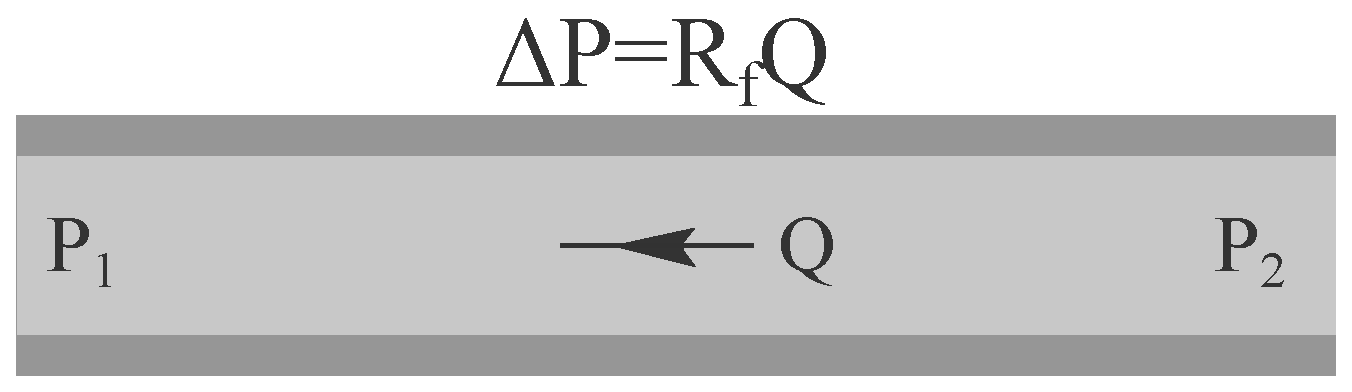
\includegraphics[width=0.45\textwidth]{immagini/poiseuille.eps}}\\
	\subfigure[]%
	{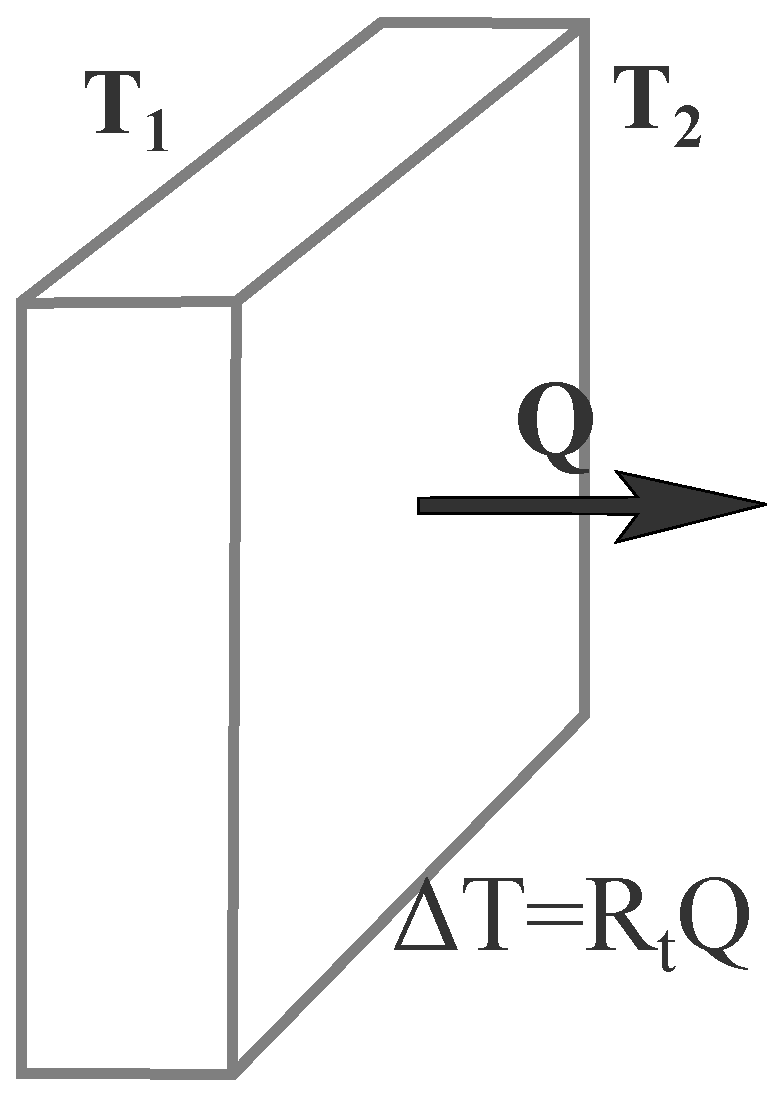
\includegraphics[width=0.25\textwidth]{immagini/fourier.eps}}\qquad
	\subfigure[]%
	{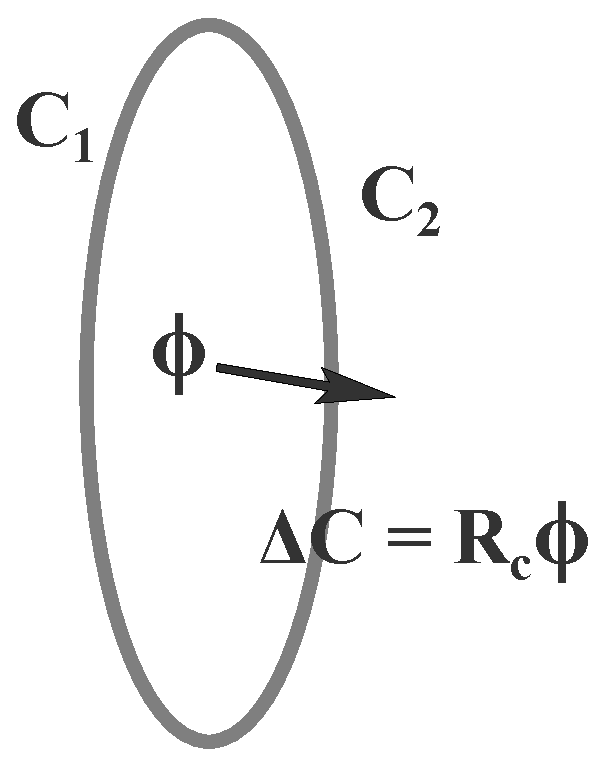
\includegraphics[width=0.27\textwidth]{immagini/fick.eps}}
	\caption{Legge di Ohm generalizzata nel caso di un sistema (a) meccanico, (b) fluidodinamico, (c) termodinamico e (d) chimico.}\label{generalized}		
\end{figure}

La seconda proprietà generalizzata dei sistemi è quella dell'\textit{accumulo}, che nei sistemi elettrici prende la forma della \textit{capacitanza}, definita come la quantità di carica elettrica $q$ accumulata nel tempo per unità di voltaggio ai capi del condensatore, cioè:
$$C = \frac{q}{V} \text{\quad con \quad} q = \int_0^t{I dt}$$
Riscrivendo il risultato in forma generalizzata si ottiene la seguente espressione:
$$\psi = \frac{1}{C}\int_0^t{\zeta}$$
Nei sistemi meccanici il termine di accumulo è chiamato \textit{compliance}. Nel caso di una molla elastica, per una data forza applicata, la compliance meccanica determina il grado con cui la molla sarà estesa o compressa. Questa proprietà è anche inversamente correlata con la \textit{rigidità}, o modulo elastico, della molla. Più la molla è compliante e più si estenderà sotto l'azione di una forza. Analogamente, in fluidodinamica, la compliance determina quanto un volume compartimentato si contrarrà o espanderà a seguito di una variazione unitaria di pressione transmurale. Nei sistemi termodinamici il termine di accumulo si identifica nella capacità termica, che dipende dalle dimensioni e dal calore specifico del mezzo di trasmissione. Infine, nei sistemi chimici, il termine di accumulo è rappresentato dal volume di solvente in cui una specie chimica è disciolta; cioè per un dato volume, la massa totale della specie chimica presente è proporzionale alla sua concentrazione, proprietà che di fatto è usata per la definizione di concentrazione.

L'ultima proprietà generalizzata dei sistemi è l'\textit{inertanza}, usata per esprimere l'accumulo di \textit{energia cinetica}. Nei sistemi elettrici è chiamata \textit{induttanza} ($L$), ed è definita come la tensione richiesta per produrre una variazione unitaria del flusso di corrente:
$$V = L \frac{dI}{dt}$$
Sostituendo $V$ e $I$ con le rispettive variabili generalizzate si ottiene:
$$\psi = L \frac{d\zeta}{dt}$$
Nel contesto della meccanica $\psi$ è la forza e $\zeta$ la velocità, così che l'equazione appena scritta altro non è che la seconda legge della dinamica di Newton: $F=m \cdot a$. In questo caso quindi l'inertanza è semplicemente la massa inerziale del sistema. L'inertanza è presente anche nei sistemi fluidodinamici in cui l'accelerazione del fluido è proporzionale alla variazione istantanea di pressione applicata. Per quanto riguarda i sistemi termici e chimici non c'è alcun elemento che rappresenti l'inertanza: in questi sistemi infatti non è possibile accumulare energia cinetica \cite{khoo}.
